\documentclass[addpoints,12pt,answers]{exam}

\usepackage{amsthm,amsfonts,amsmath,amssymb,fullpage,mathrsfs,centernot,bbm,graphicx}%,kbordermatrix
%\usepackage{matlab-prettifier,url}
\usepackage{asymptote}
\usepackage[utf8]{inputenc}
\usepackage{hyperref}
\hypersetup{colorlinks,urlcolor=blue}
\usepackage{algorithm}
\usepackage{listings}
\checkboxchar{$\Box$}
\checkedchar{$\blacksquare$}
\usepackage{multicol}
\newcommand{\tf}[1][{}]{%
  \vspace{0.1cm} \fillin[#1][0.75in]%
}
\newtheorem{theorem}{Theorem}[section]

\usepackage{lstautogobble}

\definecolor{codegreen}{rgb}{0,0.6,0}
\definecolor{codegray}{rgb}{0.5,0.5,0.5}
\definecolor{codepurple}{rgb}{0.58,0,0.82}
\definecolor{backcolour}{rgb}{0.95,0.95,0.92}

\lstset{language=Python,
    backgroundcolor=\color{backcolour},   
    commentstyle=\color{codegreen},
    keywordstyle=\color{magenta},
    numberstyle=\tiny\color{codegray},
    stringstyle=\color{codepurple},
    basicstyle=\ttfamily\footnotesize,
    breakatwhitespace=false,         
    breaklines=true,                 
    captionpos=l,                    
    keepspaces=true,                 
    numbers=left,                    
    numbersep=5pt,                  
    showspaces=false,                
    showstringspaces=false,
    showtabs=false,                  
    tabsize=1, 
    autogobble=true
}

\usepackage[noend]{algpseudocode}
\usepackage{booktabs}
\usepackage{comment,float}
\renewcommand{\phi}{\varphi}
\usepackage{caption}
\newcommand{\Range}{\ensuremath{\operatorname{\mathrm{range}}}}
\newcommand{\inputX}[1]{\input{#1}\pagebreak}
\DeclareMathOperator{\argmin}{arg\,min}
\DeclareMathOperator{\argmax}{arg\,max}
\DeclareMathOperator{\cond}{cond}
\DeclareMathOperator{\order}{order}
\DeclareMathOperator{\range}{range}
\DeclareMathOperator{\SD}{SD}
\DeclareMathOperator{\TV}{TV}
\DeclareMathOperator{\Log}{Log}
\DeclareMathOperator{\Res}{Res}
\DeclareMathOperator{\Tan}{Tan}
\DeclareMathOperator{\Arg}{Arg}
\DeclareMathOperator{\Bin}{Bin}
\DeclareMathOperator{\Ber}{Ber}
\DeclareMathOperator{\Geom}{Geom}
\DeclareMathOperator{\Gam}{Gamma}
\DeclareMathOperator{\InvGam}{InvGamma}
\DeclareMathOperator{\Bet}{Beta}
\DeclareMathOperator{\Beta}{B}
\DeclareMathOperator{\Pois}{Pois}
\DeclareMathOperator{\Norm}{\mathcal{N}}
\DeclareMathOperator{\NBin}{NBin}
\DeclareMathOperator{\HGeom}{HGeom}
\DeclareMathOperator{\Unif}{Unif}
\DeclareMathOperator{\Area}{Area}
\DeclareMathOperator{\sech}{sech}
\DeclareMathOperator{\card}{card}
\DeclareMathOperator{\Span}{Span}
\DeclareMathOperator{\im}{im}
\DeclareMathOperator{\tr}{\textbf{tr}}
\DeclareMathOperator{\diag}{\textbf{diag}}
\DeclareMathOperator{\rank}{\textbf{rank}}
\DeclareMathOperator{\dom}{\textbf{dom}}
\DeclareMathOperator{\Ind}{\mathbf{1}}
\DeclareMathOperator{\Int}{\textbf{int}}
\DeclareMathOperator{\Cl}{\textbf{cl}}
\renewcommand{\Pr}{P}
\newcommand{\E}{E}
\newcommand{\notto}{\centernot\to}
\newcommand{\Matlab}{\textsc{Matlab}~}
\newcommand{\Null}{\ensuremath{\operatorname{\mathrm{null}}}}
\newcommand{\Col}{\ensuremath{\operatorname{\mathcal{C}}}}
\newcommand{\Alt}{\ensuremath{\operatorname{Alt}}}
\newcommand{\diam}{\ensuremath{\operatorname{\mathrm{diam~}}}}
\newcommand{\sgn}{\ensuremath{\operatorname{\mathrm{sgn}}}}
\newcommand{\rref}{\ensuremath{\operatorname{\mathrm{rref}}}}
\newcommand{\ran}{\ensuremath{\operatorname{\mathrm{ran~}}}}
\newcommand{\Var}{\ensuremath{\operatorname{\mathrm{Var}}}}
\newcommand{\Cov}{\ensuremath{\operatorname{\mathrm{Cov}}}}
\newcommand{\Mor}{\ensuremath{\operatorname{\mathrm{Mor}}}}
\newcommand{\Exp}{\ensuremath{\operatorname{\mathrm{Exp}}}}
\newcommand{\Top}{\ensuremath{\operatorname{\mathrm{Top}}}}
\newcommand{\nul}{\ensuremath{\operatorname{\mathrm{nul}}}}
\newcommand{\supp}{\ensuremath{\operatorname{\mathrm{supp}}}}
\newcommand{\col}{\ensuremath{\operatorname{\mathrm{col}}}}
\newcommand{\id}{\ensuremath{\operatorname{\mathrm{id}}}}
\newcommand{\bd}{\ensuremath{\partial}}
\newcommand{\lp}{\ensuremath{\operatorname{\mathrm{lp~}}}}
\renewcommand{\Re}{\ensuremath{\operatorname{\mathrm{Re}}}}
\renewcommand{\Im}{\ensuremath{\operatorname{\mathrm{Im}}}}
\renewcommand{\AA}{\ensuremath{\mathcal{A}}}
\newcommand{\upto}{\ensuremath{\uparrow}}
\newcommand{\downto}{\ensuremath{\downarrow}}
\newcommand{\ind}{\ensuremath{\mathbf{1}}}
\newcommand{\cc}{\ensuremath{\mathfrak{c}}}
\newcommand{\XX}{\ensuremath{\mathcal{X}}}
\newcommand{\YY}{\ensuremath{\mathcal{Y}}}
\newcommand{\RR}{\ensuremath{\mathbb{R}}}
\newcommand{\RRb}{\ensuremath{\overline{\RR}}}
\newcommand{\RRR}{\ensuremath{\mathcal{R}}}
\newcommand{\AAA}{\ensuremath{\mathcal{A}}}
\newcommand{\MMM}{\ensuremath{\mathcal{M}}}
\newcommand{\FF}{\ensuremath{\mathcal{F}}}
\newcommand{\FFF}{\ensuremath{\mathcal{F}}}
\newcommand{\VVV}{\ensuremath{\mathscr{V}}}
\newcommand{\EE}{\ensuremath{\mathscr{E}}}
\newcommand{\EEE}{\ensuremath{\mathcal{E}}}
\newcommand{\DD}{\ensuremath{\mathcal{D}}}
\newcommand{\QQ}{\ensuremath{\mathbb{Q}}}
\newcommand{\NQ}{\ensuremath{\mathbb{I}}}
\newcommand{\NN}{\ensuremath{\mathbb{N}}}
\newcommand{\NNN}{\ensuremath{\mathcal{N}}}
\newcommand{\ZZ}{\ensuremath{\mathbb{Z}}}
\newcommand{\ZZZ}{\ensuremath{\mathcal{Z}}}
\newcommand{\CC}{\ensuremath{\mathbb{C}}}
\newcommand{\CCC}{\ensuremath{\mathcal{C}}}
\newcommand{\HH}{\ensuremath{\mathbb{H}}}
\newcommand{\NNb}{\ensuremath{\mathbb{\overline{N}}}}
\newcommand{\RRc}{\ensuremath{\mathcal{R}}}
\newcommand{\OO}{\ensuremath{\mathcal{O}}}
\newcommand{\II}{\ensuremath{\mathscr{I}}}
\newcommand{\JJ}{\ensuremath{\mathscr{J}}}
\newcommand{\BB}{\ensuremath{\mathcal{B}}}
\newcommand{\BBB}{\ensuremath{\mathcal{B}}}
\newcommand{\TT}{\ensuremath{\mathbb{T}}}
\newcommand{\TTT}{\ensuremath{\mathcal{T}}}
\newcommand{\LL}{\ensuremath{\mathcal{L}}}
\newcommand{\LLL}{\ensuremath{\mathcal{L}}}
\newcommand{\WW}{\ensuremath{\mathcal{W}}}
\newcommand{\UU}{\ensuremath{\mathcal{U}}}
\newcommand{\UUU}{\ensuremath{\mathcal{U}}}
\renewcommand{\SS}{\ensuremath{\mathcal{S}}}
\newcommand{\Mod}[1]{\ensuremath{\mbox{ (mod $#1$)}}}
\newcommand{\PP}{\ensuremath{P}}
\newcommand{\PPP}{\ensuremath{\mathcal{P}}}
\newcommand{\POL}{\ensuremath{\mathcal{P}}}
\newcommand{\GG}{\ensuremath{\mathcal{G}}}
\newcommand{\Pow}[1]{\ensuremath{\PP(#1)}}
\newcommand{\rel}{\ensuremath{\mathbin{\mbox{rel}}}}
\newcommand{\SimpSet}[1]{\ensuremath{\{\,#1\,\}}}
\newcommand{\BSimpSet}[1]{\ensuremath{\left\{\,#1\,\right\}}}
\newcommand{\BSimpList}[1]{\ensuremath{\left(\,#1\,\right)}}
\newcommand{\BSet}[2]{\ensuremath{\{\,#1\mid #2\,\}}}
\newcommand{\Gen}[2]{\ensuremath{\langle\,#1\mid #2\,\rangle}}
\newcommand{\Set}[2]{\ensuremath{\left\{\,#1\left\vert\vphantom{\left\{#1#2\right.}\right.#2\,\right\}}}
\newcommand{\Sol}{\textit{Solution. }}
\newcommand{\Not}{\textit{Notes. }}
\newenvironment{idea}{\medbreak\noindent\textit{Idea.}}{}
\newenvironment{sketch}{\medbreak\noindent\textit{Proof sketch.}}{}
\ifdefined\USESOLUTIONS
  \includecomment{solution}
\else
  \excludecomment{solution}
\fi
\newenvironment{Array}{
  \everymath{\displaystyle\everymath{}}
  \setlength\arraycolsep{8pt}
  \def\arraystretch{2}
  \array
}
{
  \endarray
}

\newcommand{\Mat}[3]{\left(\begin{array}{c}#1\\#2\\#3\end{array}\right)}
\newcommand{\Mas}[2]{\left(\begin{array}{c}#1\\#2\end{array}\right)}
\newcommand{\Matt}[4]{\left(\begin{array}{cc}#1&#2\\#3&#4\end{array}\right)}
\newcommand{\MATT}[4]{\left(\begin{Array}{cc}#1&#2\\#3&#4\end{Array}\right)}
\newcommand{\Matts}[6]{\left(\begin{array}{ccc}#1&#2&#3\\#4&#5&#6\end{array}\right)}
\newcommand{\Mattt}[9]{\left(\begin{array}{ccc}#1&#2&#3\\#4&#5&#6\\#7&#8&#9\end{array}\right)}
\newcommand{\PMat}[1]{\left(\begin{Array}{cccccccc}#1\end{Array}\right)}
\newcommand{\PMatt}[2]{\left(\begin{Array}{cccccccc}#1\\#2\end{Array}\right)}
\newcommand{\PMattt}[3]{\left(\begin{Array}{cccccccc}#1\\#2\\#3\end{Array}\right)}
\newcommand{\PMatttt}[4]{\left(\begin{Array}{cccccccc}#1\\#2\\#3\\#4\end{Array}\right)}
\newcommand{\PMattttt}[5]{\left(\begin{Array}{cccccccc}#1\\#2\\#3\\#4\\#5\end{Array}\right)}
\newcommand{\PMatttttt}[6]{\left(\begin{Array}{cccccccc}#1\\#2\\#3\\#4\\#5\\#6\end{Array}\right)}
\newcommand{\pMat}[1]{\left(\begin{array}{cccccccc}#1\end{array}\right)}
\newcommand{\pMatt}[2]{\left(\begin{array}{cccccccc}#1\\#2\end{array}\right)}
\newcommand{\pMattt}[3]{\left(\begin{array}{cccccccc}#1\\#2\\#3\end{array}\right)}
\newcommand{\pMatttt}[4]{\left(\begin{array}{cccccccc}#1\\#2\\#3\\#4\end{array}\right)}
\newcommand{\pMattttt}[5]{\left(\begin{array}{cccccccc}#1\\#2\\#3\\#4\\#5\end{array}\right)}
\newcommand{\pMatttttt}[6]{\left(\begin{array}{cccccccc}#1\\#2\\#3\\#4\\#5\\#6\end{array}\right)}
\newcommand{\Diagg}[2]{\PMatt{#1&0}{0&#2}}
\newcommand{\Diaggg}[3]{\PMattt{#1&0&0}{0&#2&0}{0&0&#3}}
\newcommand{\Diagggg}[4]{\PMatttt{#1&0&0&0}{0&#2&0&0}{0&0&#3&0}{0&0&0&#4}}
\newcommand{\Diaggggg}[5]{\PMattttt{#1&0&0&0&0}{0&#2&0&0&0}{0&0&#3&0&0}{0&0&0&#4&0}{0&0&0&0&#5}}
\newcommand{\diagg}[2]{\pMatt{#1&0}{0&#2}}
\newcommand{\diaggg}[3]{\pMattt{#1&0&0}{0&#2&0}{0&0&#3}}
\newcommand{\diagggg}[4]{\pMatttt{#1&0&0&0}{0&#2&0&0}{0&0&#3&0}{0&0&0&#4}}
\newcommand{\diaggggg}[5]{\pMattttt{#1&0&0&0&0}{0&#2&0&0&0}{0&0&#3&0&0}{0&0&0&#4&0}{0&0&0&0&#5}}

\newcommand*{\horzbar}{\rule[.5ex]{2.5ex}{0.5pt}}


\global\long\def\reals{\mathbf{R}}
\global\long\def\integers{\mathbf{Z}}
\global\long\def\naturals{\mathbf{N}}
\global\long\def\rationals{\mathbf{Q}}
\global\long\def\ca{\mathcal{A}}
\global\long\def\cb{\mathcal{B}}
\global\long\def\cc{\mathcal{C}}
\global\long\def\cd{\mathcal{D}}
\global\long\def\ce{\mathcal{E}}
\global\long\def\cf{\mathcal{F}}
\global\long\def\cg{\mathcal{G}}
\global\long\def\ch{\mathcal{H}}
\global\long\def\ci{\mathcal{I}}
\global\long\def\cj{\mathcal{J}}
\global\long\def\ck{\mathcal{K}}
\global\long\def\cl{\mathcal{L}}
\global\long\def\cm{\mathcal{M}}
\global\long\def\cn{\mathcal{N}}
\global\long\def\co{\mathcal{O}}
\global\long\def\cp{\mathcal{P}}
\global\long\def\cq{\mathcal{Q}}
\global\long\def\calr{\mathcal{R}}
\global\long\def\cs{\mathcal{S}}
\global\long\def\ct{\mathcal{T}}
\global\long\def\cu{\mathcal{U}}
\global\long\def\cv{\mathcal{V}}
\global\long\def\cw{\mathcal{W}}
\global\long\def\cx{\mathcal{X}}
\global\long\def\cy{\mathcal{Y}}
\global\long\def\cz{\mathcal{Z}}
\global\long\def\ind#1{1(#1)}
\global\long\def\pr{\mathbb{P}}
\global\long\def\predsp{\cy}
\global\long\def\outsp{\cy}
\global\long\def\prxy{P_{\cx\times\cy}}
\global\long\def\prx{P_{\cx}}
\global\long\def\prygivenx{P_{\cy\mid\cx}}
\global\long\def\ex{\mathbb{E}}
\global\long\def\var{\textrm{Var}}
\global\long\def\cov{\textrm{Cov}}
\global\long\def\sgn{\textrm{sgn}}
\global\long\def\sign{\textrm{sign}}
\global\long\def\kl{\textrm{KL}}
\global\long\def\law{\mathcal{L}}
\global\long\def\eps{\varepsilon}
\global\long\def\as{\textrm{ a.s.}}
\global\long\def\io{\textrm{ i.o.}}
\global\long\def\ev{\textrm{ ev.}}
\global\long\def\convd{\stackrel{d}{\to}}
\global\long\def\eqd{\stackrel{d}{=}}
\global\long\def\del{\nabla}
\global\long\def\loss{V}
\global\long\def\risk{R}
\global\long\def\emprisk{\hat{R}_{\ell}}
\global\long\def\lossfnl{L}
\global\long\def\emplossfnl{\hat{L}}
\global\long\def\empminimizer#1{\hat{#1}_{\ell}}
\global\long\def\minimizer#1{#1_{*}}
\global\long\def\etal{\textrm{et. al.}}
\global\long\def\tr{\operatorname{tr}}
\global\long\def\trace{\operatorname{trace}}
\global\long\def\diag{\text{diag}}
\global\long\def\rank{\text{rank}}
\global\long\def\linspan{\text{span}}
\global\long\def\proj{\text{Proj}}
%\global\long\def\argmax{\operatornamewithlimits{arg\, max}}
%\global\long\def\argmin{\operatornamewithlimits{arg\, min}}
\global\long\def\bfx{\mathbf{x}}
\global\long\def\bfy{\mathbf{y}}
\global\long\def\bfl{\mathbf{\lambda}}
\global\long\def\bfm{\mathbf{\mu}}
\global\long\def\calL{\mathcal{L}}
\global\long\def\vw{\boldsymbol{w}}
\global\long\def\vx{\boldsymbol{x}}
\global\long\def\vxi{\boldsymbol{\xi}}
\global\long\def\valpha{\boldsymbol{\alpha}}
\global\long\def\vbeta{\boldsymbol{\beta}}
\global\long\def\vsigma{\boldsymbol{\sigma}}
\global\long\def\vmu{\boldsymbol{\mu}}
\global\long\def\vtheta{\boldsymbol{\theta}}
\global\long\def\vd{\boldsymbol{d}}
\global\long\def\vs{\boldsymbol{s}}
\global\long\def\vt{\boldsymbol{t}}
\global\long\def\vh{\boldsymbol{h}}
\global\long\def\ve{\boldsymbol{e}}
\global\long\def\vf{\boldsymbol{f}}
\global\long\def\vg{\boldsymbol{g}}
\global\long\def\vz{\boldsymbol{z}}
\global\long\def\vk{\boldsymbol{k}}
\global\long\def\va{\boldsymbol{a}}
\global\long\def\vb{\boldsymbol{b}}
\global\long\def\vv{\boldsymbol{v}}
\global\long\def\vy{\boldsymbol{y}}
\global\long\def\hil{\ch}
\global\long\def\rkhs{\hil}
 


\begin{document}
\pagestyle{foot}
\footer{}{Page \thepage\ of \numpages}{}

\begin{coverpages}

  \begin{center}
    {\LARGE DS-GA-1003: Machine Learning (Spring 2020) }\\
    \vspace{0.2in}
    {\LARGE Midterm Exam (March 10 5:20-11:59PM)}
    \vspace{0.1in}

\fbox{\fbox{\parbox{6.5in}{\centering 
\begin{itemize}
  \item While the exam should take 90 minute, you have until \textbf{11:59PM on} \newline  \textbf{Tuesday March 10} to submit your answers on Gradescope. You have until \newline 11:59PM on Wednesday March 11 for late submissions. 
    \item No textbooks, notes, online resources or calculators. However you are allowed \newline a double-sided reference sheet.
    \item The exam consists of \numpages \, pages. If you are annotating the exam, then mark your answers in the provided space.  If you lack space for an answer, then use the blank space on page \numpages. If you are typing your responses, then please follow the directions on Piazza. 
\end{itemize}

}}}
  \end{center}

  \vspace{0.4in}
  \makebox[\textwidth]{Name:\enspace\hrulefill}

  \vspace{10mm}


  \makebox[\textwidth]{NYU NetID:\enspace\hrulefill}
  \vspace{5mm}

  \makebox[\textwidth]{NYU Email:\enspace\hrulefill}
\indent 
 
    \vspace{-0.00in}
 
  \begin{center}
    \gradetable[v][questions]
  \end{center}
  

\end{coverpages}

\begin{questions}

\titledquestion{Decomposing Risk} Consider input space $\XX$, output space $\YY$ and action space $\mathcal{A}$. Fix a loss function $\ell$ on $\mathcal{A} \times \YY$. Consider hypothesis space $\FF$ of functions from $\XX$ to $\mathcal{A}$. Fix a sample $S$ drawn from $\XX \times \YY$. Take
  \vspace{-0.2in}
  \begin{flushright}
      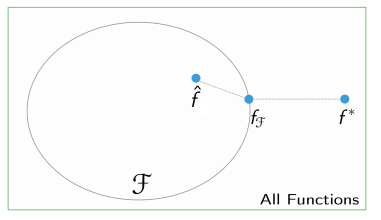
\includegraphics[width=6cm,height=4cm]{risk_decomp.PNG}
    \end{flushright}

\vspace{-1.6in}    
  \begin{itemize}
      \item $f^* = \underset{f}{\operatorname{argmin}} \; \mathbb{E}\left[\ell(f(x),y)\right]$
    \item $f_{\mathcal{F}} = \underset{f \in \mathcal{F}}{\operatorname{argmin}} \; \mathbb{E}\left[\ell(f(x),y)\right]$
    \item $\hat{f} = \underset{f \in \mathcal{F}}{\operatorname{argmin}} \; \frac{1}{m} \sum_{i=1}^{m} \ell(f(x_i), y_i)$ \newline 
    \vspace{0.1cm}
    
    {\hspace{-0.9cm} where $m$ is the number of samples in $S$.}
  \end{itemize}

\vspace{0.2in}  

  \begin{parts}
  \part Recall that the approximation error is the difference of risks $R(f_{\mathcal{F}}) - R(f^*)$.  
\vspace{0.1in}

\begin{subparts}
\subpart[1] The approximation error is 
\vspace{0.1in}
\newline
  \begin{oneparcheckboxes}
    \choice Positive or Zero
    \choice Negative or Zero
    \choice Cannot be Determined
    \end{oneparcheckboxes}
\subpart[1] The approximation error is
\vspace{0.1in}
\newline
  \begin{oneparcheckboxes}
    \choice Random
    \choice Non-Random
    \choice Cannot be Determined
    \end{oneparcheckboxes}
\subpart[1] If we increase the size of $\FF$, then the approximation error is
 \vspace{0.1in}
\newline
  \begin{oneparcheckboxes}
    \choice Increased or Unchanged 
    \choice Decreased or Unchanged
    \newline \choice Cannot be Determined
    \end{oneparcheckboxes}
\subpart[1] If we increase the size of $S$, then the approximation error is
  \vspace{0.1in}
\newline
  \begin{oneparcheckboxes}
    \choice Changed 
    \choice Unchanged 
    \choice Cannot be Determined
    \end{oneparcheckboxes}
\subpart[1] Do we need to know the data generating distribution to compute the approximation error? 
  \vspace{0.05in}
\newline
  \begin{oneparcheckboxes}
    \choice True
    \choice False
    \end{oneparcheckboxes}
\end{subparts}


\part Recall that the estimation error is the difference of risks $R(\hat{f}) - R(f_{\mathcal{F}})$.  
\vspace{0.1in}

\begin{subparts}
\subpart[1] The estimation error is
\vspace{0.1in}
\newline
  \begin{oneparcheckboxes}
    \choice Positive or Zero
    \choice Negative or Zero 
    \choice Cannot be Determined
    \end{oneparcheckboxes}
\subpart[1] For fixed sample $S$, the estimation error is 
\vspace{0.1in}
\newline
  \begin{oneparcheckboxes}
    \choice Random
    \choice Non-Random
    \choice Cannot be Determined
    \end{oneparcheckboxes}
\subpart[1] If we increase the size of $\FF$, then the estimation error is
 \vspace{0.1in}
\newline
  \begin{oneparcheckboxes}
    \choice Increased or Unchanged 
    \choice Decreased or Unchanged
    \newline \choice Cannot be Determined
    \end{oneparcheckboxes}
\subpart[1] If we increase the size of $S$, then the estimation error is
  \vspace{0.1in}
\newline
  \begin{oneparcheckboxes}
    \choice Changed  
    \choice Unchanged
    \choice Cannot be Determined
    \end{oneparcheckboxes}
\subpart[1] Do we need to know the data generating distribution to compute approximation error 
  \vspace{0.1in}
\newline
  \begin{oneparcheckboxes}
    \choice True
    \choice False
    \end{oneparcheckboxes}
\end{subparts}
  \vspace{0.1in}
\part[1] For some models like Lasso Regression, we have different approaches to fitting the training data. Each approach attempts to find $\widehat{f}$. Does the choice of the approach affect 
  \vspace{0.0in}
\newline

  \begin{oneparcheckboxes}
    \choice Approximation Error
    \choice Estimation Error 
    \choice Neither 
    \end{oneparcheckboxes}

  \end{parts}

\titledquestion{Regularization} 
\begin{parts}
    
\part We have a dataset $\cd=\left\{ \left(0,1\right),(1,4),(2,3)\right\} $
that we fit by minimizing an objective function of the form:
\[
J(\alpha_{0},\alpha_{1})=\lambda_{1}\left(\alpha_{0}+\alpha_{1}\right)+\lambda_{2}(\alpha_{0}^{2}+\alpha_{1}^{2}) + \sum_{i=1}^{3}\left(\alpha_{0}+\alpha_{1}x_{i}-y_{i}\right)^{2},
\]
and the corresponding fitted function is given by $f(x)=\alpha_{0}+\alpha_{1}x$.
We tried four different settings of $\lambda_{1}$ and $\lambda_{2}$,
and the results are shown below. 

\begin{figure}[h]
\centering{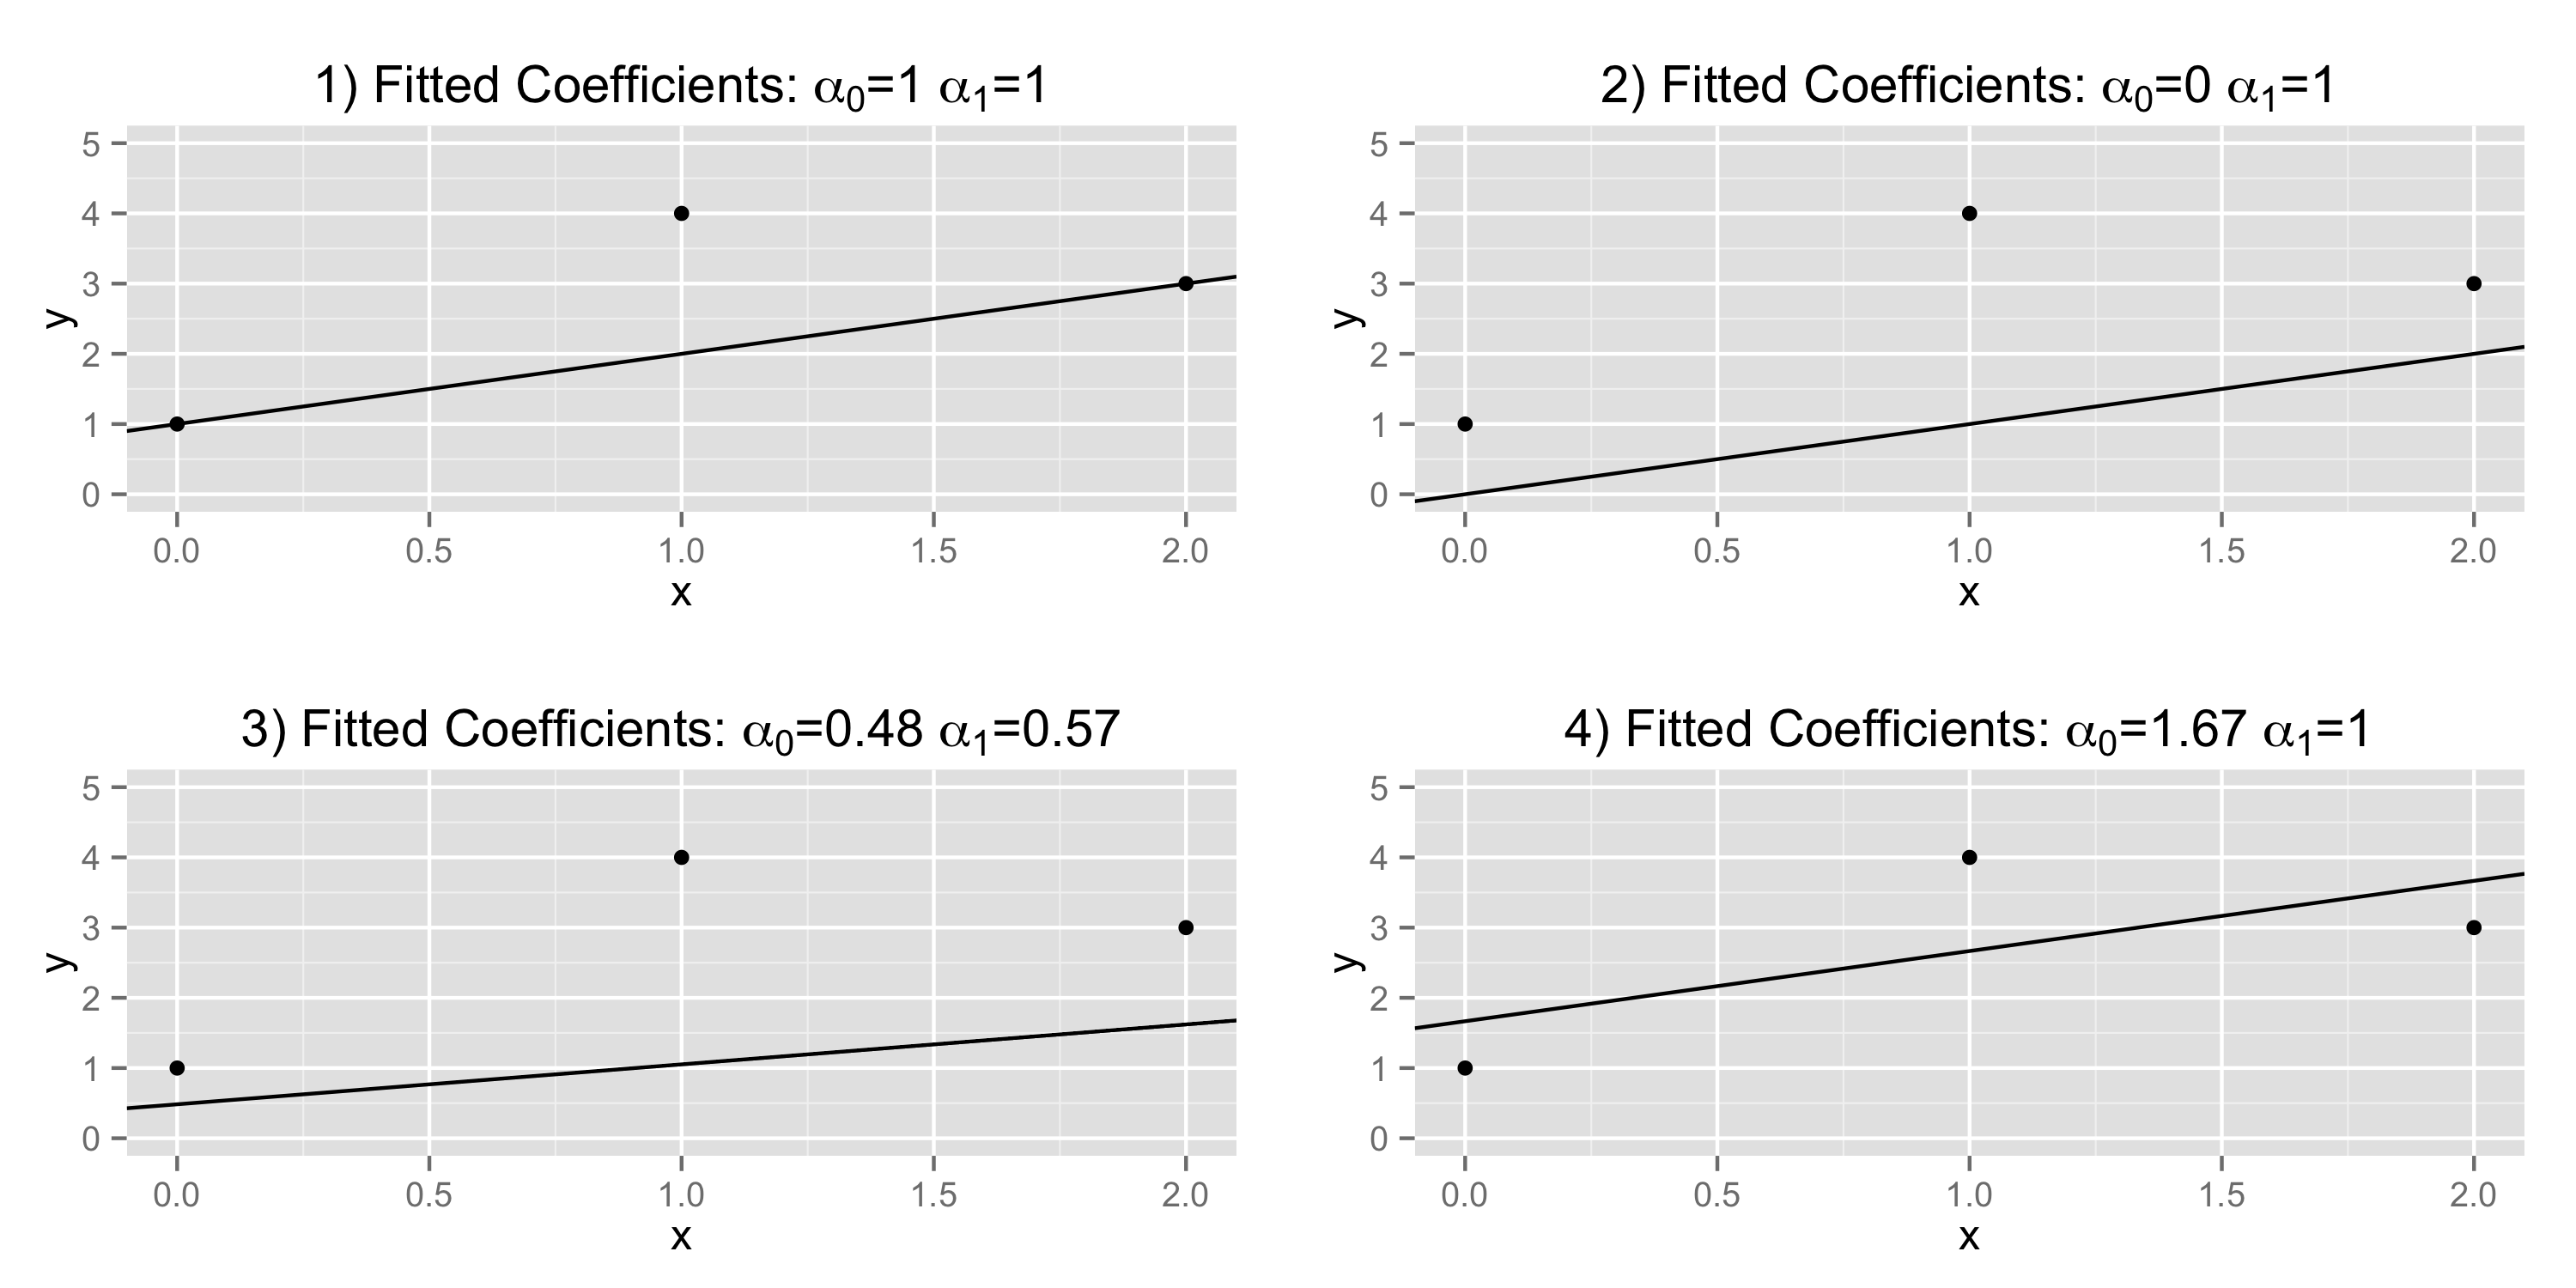
\includegraphics[width=6in, height=2.8in]{fourFits.png}}
\end{figure}
For each of the following parameter settings, give the number of the plot that
shows the resulting fit.

\begin{subparts}
    \subpart[2]  \tf[ ] $\lambda_{1}=0$ and $\lambda_{2}=2$. 
 \subpart[2] \tf[ ] $\lambda_{1}=0$ and $\lambda_{2}=0$.
\subpart[2] \tf[ ] $\lambda_{1}=0$ and $\lambda_{2}=10$.
\subpart[2] \tf[ ] $\lambda_{1}=5$ and $\lambda_{2}=0$.
\end{subparts}


\end{parts}
 
\titledquestion{Scaling} Suppose we have input space $\XX=\left\{-1.5,-0.5,0.5,1.5 \right\} \times \left\{ -0.001, 0.001 \right\}$, output space $\YY =  \left\{ -1, 1 \right\}$ and action space $\mathbb{R}$. Assume the following about the data generating distribution 
\begin{itemize}
    \item $Y$ coordinate has equal probability of being $-1,1$
    \item $X_1$ coordinate has equal probability of being $\left\{-1.5,-0.5,0.5,1.5 \right\}$. $X_1$ is related to $Y$ through $X_1 = Y - 0.5 Z$ where $Z = \pm 1$ with equal probability
    \item $X_2$ has equal probability of being $\left\{-0.001,0.001 \right\}$. $X_2$ is related to $Y$ through $X_2 = Y / 1000$
\end{itemize}
Suppose we have Ridge Regression with $m$ samples 
\[
J(\mathbf{w})=\lambda(w_{1}^{2}+w_{2}^{2}) + \frac{1}{m}\sum_{i=1}^{m}\left(w_{1}x^{(i)}_{1}+w_{2}x^{(i)}_{2}-y_{i}\right)^{2}
\]
We're trying to decide between weights $\mathbf{w}_{\operatorname{accurate}} = \left[0, 1000\right]$ and $\mathbf{w}_{\operatorname{small}} = \left[1, 0\right]$. 
\begin{parts}
    \part[2] What is the value of $J(\mathbf{w}_{\operatorname{accurate}})$? 
    \vspace{0.1in}
    
    \begin{oneparcheckboxes}
\choice $1000 \lambda$
\choice $1000$
\choice $1000^2 \lambda$
\choice $1000^2$
\end{oneparcheckboxes}
    \part[2] For large values of $m$, the empirical risk $$\frac{1}{m}\sum_{i=1}^{m}\left(w_{1}x^{(i)}_{1}+w_{2}x^{(i)}_{2}-y_{i}\right)^{2}$$ approximates the statistical risk $$\mathbb{E}\left[\left(w_1 X_1 + w_2 X_2 - Y \right)^2\right] \, .$$ Use the statistical risk to approximate the value $J(\mathbf{w}_{\operatorname{small}})$. 
        \vspace{0.1in}
        
    \begin{oneparcheckboxes}
\choice $0.5 + \lambda$
\choice $0.25 + \lambda$
\choice $1 + \lambda$
\choice $0.75 + \lambda$
\end{oneparcheckboxes}
    \part[2] Using your answers above, determine $\lambda^*$ such that we would choose $\mathbf{w}_{\operatorname{small}}$ for any $\lambda > \lambda^*$.
    \begin{solutionorbox}[1.5in]
         
    \end{solutionorbox}
\newpage
    \part[2] For most values of $\lambda$, we would choose $\mathbf{w}_{\operatorname{small}}$. How could we transform the features to avoid choosing the less accurate weights?
    \begin{solutionorbox}[1in]
          
    \end{solutionorbox}
\end{parts}

\titledquestion{Gradient Descent}

Momentum is a variation of gradient descent where we include the gradient at a previous iteration in the current iteration. The update rule is 

$$\mathbf{w}^{(t+1)} = \mathbf{w}^{(t)} - \alpha \frac{\partial L}{\partial \mathbf{w}} \left(\mathbf{w}^{(t)}\right) - \gamma \frac{\partial L}{\partial \mathbf{w}}\left(\mathbf{w}^{(t-1)}\right)$$

Here $L$ is the objective function and $\alpha, \gamma > 0$ are the learning rates. Assume for iteration $t=0$ and $t=-1$, we set $\mathbf{w}^{(t)} = w_0 $  the initial guess.
\begin{figure}[h]
  \begin{minipage}[c]{0.8\textwidth}
\centering{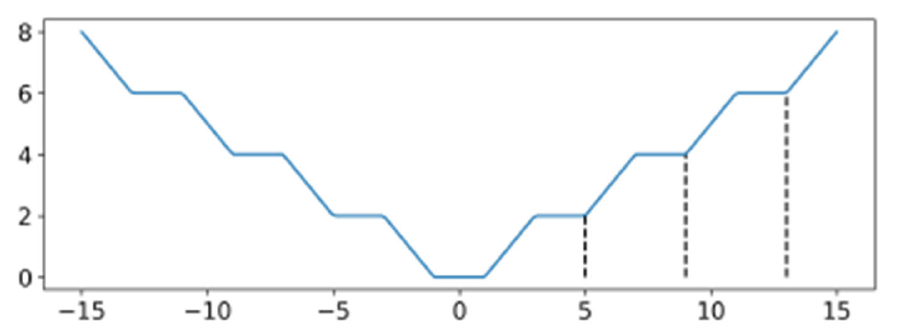
\includegraphics[scale=0.5]{gd.PNG}}
  \end{minipage}\hfill
  \begin{minipage}[c]{0.2\textwidth}
\caption{Graph of objective function $L$}
  \label{fig:gd}
  \end{minipage}
\end{figure}

\begin{parts}
\part Refer to the chart in Figure \ref{fig:gd}.
\begin{subparts}
\subpart[1] Assuming that $\mathbf{w}$ starts in a flat region that is not a minimum and $\alpha > 0$, will the basic gradient descent algorithm terminate at a minimum? Note that the basic gradient descent algorithm is the momentum gradient descent algorithm with $\gamma = 0$
\newline

\vspace{-0.3cm}
\begin{oneparcheckboxes}
\choice Yes with enough iterations 
\choice Maybe 
\choice Never 
\end{oneparcheckboxes}
\vspace{0.1cm}
\subpart[1] Assuming that $\mathbf{w}$ starts in a sloped region and $\alpha > 0$, will the basic gradient descent algorithm terminate at a minimum? 
\newline

\vspace{-0.3cm}
\begin{oneparcheckboxes}
\choice Yes with enough iterations 
\choice Maybe 
\choice Never 
\end{oneparcheckboxes}
\vspace{0.1cm}
\subpart[1] Assuming that $\mathbf{w}$ starts in a flat region that is not a minimum and both $\alpha > 0$ and $\gamma > 0$, will the momentum gradient descent algorithm terminate at a minimum? 
\newline

\vspace{-0.3cm}
\begin{oneparcheckboxes}
\choice Yes with enough iterations 
\choice Maybe 
\choice Never 
\end{oneparcheckboxes}
\vspace{0.1cm}
\subpart[1] Assuming that $\mathbf{w}$ starts in a sloped region  and both $\alpha > 0$ and $\gamma > 0$, will the momentum gradient descent algorithm terminate at a minimum? 
\newline

\vspace{-0.2cm}
\begin{oneparcheckboxes}
\choice Yes with enough iterations 
\choice Maybe 
\choice Never 
\end{oneparcheckboxes}

\vspace{0.1cm}
\subpart[1] Is $L(\mathbf{w})$ convex?
\newline
\vspace{-0.1cm}

\begin{oneparcheckboxes}
\choice Yes
\choice No
\choice No, but $-L(\mathbf{w})$ is convex
\choice No, but $L(-\mathbf{w})$ is convex
\end{oneparcheckboxes}
\end{subparts}
\vspace{0.6cm}

\part[6] Fill in the twelve blanks in the code with the following variables to implement gradient descent with momentum.  
\vspace{0.1in}
\newline

\centering{

\begin{tabular}{|l|l|l|l|l|1|}
\hline
w                & X                & y              & w\_prev       & num\_iter    & w0\\ \hline
temp                  & alpha              & gamma          & range             & len &  t \\ \hline
\end{tabular}
}
\vspace{0.1in}
\newline
\begin{flushleft}
Note that the same variable can be used multiple times. Some variables may not be used at all. Only use one variable per blank.
\end{flushleft}

\begin{lstlisting}
def grad(X, y, w):
    ''' Returns gradient dL/dw at w 
    X: matrix, training data features
    y: vector, training data labels
    w: vector, weights '''
    
def grad_desc_momentum(X, y, num_iter, alpha, gamma, w0):
    ''' Returns weights w computed after num_iter iterations.
    X: matrix, training data features
    y: vector, training data labels
    num_iter: number, number of iterations to run
    alpha: number, learning rate
    gamma: number, learning rate for momentum
    w0: weights for t=0 and t=-1 '''
    
    w, w_prev = ______<i>_______, ______<ii>______
    for ___<iii>_____ in ____<iv>____(_________<v>_______):
        g = grad(X, y, w)
        m = grad(X, y, ______<vi>_____)
        __<vii>___, ___<viii>___ = ___<ix>____ - ___<x>___ * g \ 
                                   - __<xi>___ * m, ____<xii>___
    return w
\end{lstlisting}

\vspace{0.3cm}
\begin{multicols}{3}
\begin{subparts}
\subpart \tf[ ]
\subpart \tf[ ]
\subpart \tf[ ]
\subpart \tf[ ]
\subpart \tf[ ]
\subpart \tf[ ]
\subpart \tf[ ]
\subpart \tf[ ]
\subpart \tf[ ]
\subpart \tf[ ]
\subpart \tf[ ]
\subpart \tf[ ]
\end{subparts}
\end{multicols}

\end{parts}


  \titledquestion{Loss Functions} \\
  
  Consider input space $\XX=\{1,2,3,4\}$, output space $\YY=\{1,2,3,4\}$ and action space $\mathbb{R}$. Take the square loss:    $\ell(\hat{y},y)=(\hat{y}-y)^2$.

      \begin{parts}
     \part[3] Fix $x$. Determine the constant $c$ such that $\mathbb{E}\left[(Y - c)^2 | X = x \right]$ is minimized. Note that you need to take a derivative.
\begin{solutionorbox}[1in]
      
\end{solutionorbox}
  
      \part[3]  Assume the following about the data generating distribution 
    \begin{itemize}
        \item The coordinate $X$ is uniformly distributed on $\mathcal{X}$. So equal probability $\frac{1}{4}$ to features $\{1,2,3,4\}$.  
        \item The coordinate $Y$ given the coordinate $X$ is uniformly distributed on $\{1,\ldots,x\}$. So equal probabilities $\frac{1}{x}$ to labels $\{1,\ldots,x\}$ conditional on feature $x$. 
    \end{itemize} 
 What is the target function? In other words, for fixed $x$ how should we choose $f^*(x)$ to minimize the expected square loss. 
      \begin{solutionorbox}[1in]
        
      \end{solutionorbox}
      
      \part[4] What is the expected square loss of the target function?
      \begin{solutionorbox}[2in]
        
      \end{solutionorbox}
           
    \end{parts}
\titledquestion{Decision Boundaries}

\begin{parts}
\part[2] Figure \ref{fig:svm1} contains a training set $\{x_1, x_2,\ldots, x_{25}\}$. Below we have several feature transformations. By themselves, which might allow us to separate the transformed data with a linear decision boundary? Select \textbf{all} possible choices. 
\begin{figure}[h]
  \begin{minipage}[c]{0.9\textwidth}
\centering{  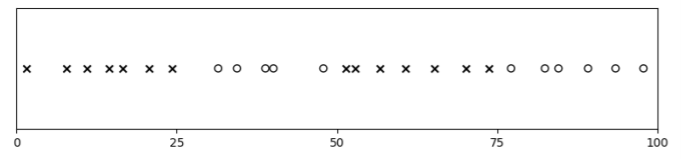
\includegraphics{svm1.PNG} }
  \end{minipage}\hfill
  \begin{minipage}[c]{0.1\textwidth}
\caption{Training Data}
  \label{fig:svm1}
  \end{minipage}
\end{figure}
\newpage
\begin{checkboxes}
\choice Centering the data
\choice Add a feature $x^2$
\choice Add a feature that is 1 if $x \leq 50$ or $-1$ if $x>50$
\choice Add two features $x^2$ and $x^3$
\end{checkboxes}
 \begin{minipage}{0.33\textwidth}
\part[2] Figure \ref{fig:svm2} contains \newline a training set \newline $\{(x^{(1)}_1,x^{(1)}_2),\ldots, (x_1^{(100)},x_2^{(100)})\}$. Below we have several feature transformations. By themselves, which might allow us to separate the transformed data with a linear decision boundary? Select \textbf{all} possible choices.  
\end{minipage}
\begin{minipage}{0.6\textwidth}
\begin{center}
    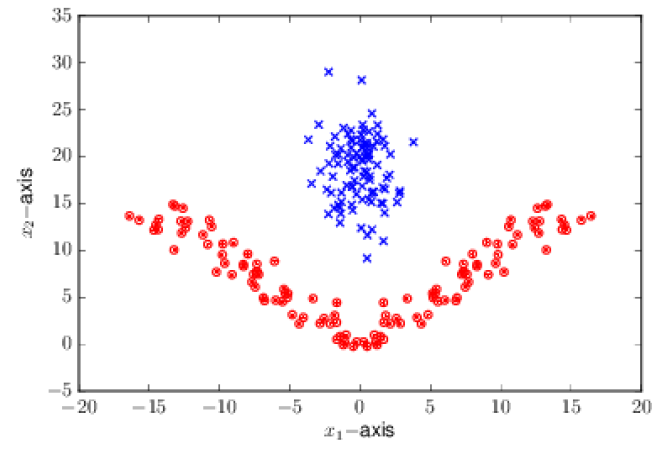
\includegraphics[scale=0.5]{dec.PNG}
    \captionof{figure}{Training Data}
\label{fig:svm2}
\end{center}
\end{minipage}


\vspace{-0.5cm}
\begin{checkboxes}
\choice Scaling the data
\choice Adding features $x_{1}^2$, $x_2^2$, $x_1x_2$
\choice Adding a feature that is 1 if $x_2 \geq 10$ or $-1$ if $x_2<10$
\choice Adding a feature $|x_1|$
\end{checkboxes}
\end{parts}
\vspace{0.3cm}

\titledquestion{Kernels}
Define the Huber loss function $h:\RR\to\RR$ by
  $$h(x) = \left\{\begin{array}{ll} x^2/2 &\text{if $|x|\leq
  1$,}\\ |x| - 1/2 & \text{if $|x|>1$.}\end{array}\right.$$
  Consider the objective function
  $$J(w) =  \lambda\|w\|_2^2 + \frac{1}{n}\sum_{i=1}^n h(w^Tx_i-y_i)$$
  where $(x_1,y_1),\ldots,(x_n,y_n)\in\RR^d\times\RR$. Fix $\lambda>0$. Note that the function is differentiable. 
  \begin{parts}
\part[3] We want to minimize $J(w)$ using stochastic gradient
    descent.  Assume the current data point is $(x_i,y_i)$.  The 
    step direction is given by $v = -\nabla_w G(w)$, for some function $G(w)$.
    Give an explicit expression for $G(w)$ in terms of $h$, $\lambda$,
    and the given data. You do not have to expand the function $h$.
    \begin{solutionorbox}[1.2in]
      
    \end{solutionorbox}
  \part[3] Assume $J(w)$ has a minimizer $w^*$.  Give an expression for
    $w^*$ in terms of a vector $\alpha\in\RR^n$
    that is guaranteed by the representer theorem.  You may use the
    design matrix $X\in\RR^{n\times d}$.
    \begin{solutionorbox}[1.2in]
      
    \end{solutionorbox}
    \part[3] Let $k:\RR^d\times\RR^d\to\RR$ be a Mercer kernel, and let
    $K\in\RR^{n\times n}$ denote the Gram matrix  $K_{ij}=k(x_i,x_j)$.
    Give a kernelized form of the objective $J$ in terms of $K$. Recall that
      $w^Tx_i = (Xw)_i$ where $X\in\RR^{n\times d}$ is the matrix with
      $i$th row $x_i^T$.
    \begin{solutionorbox}[1.5in]

    \end{solutionorbox}
  \end{parts}


\titledquestion{SVM}

\begin{minipage}{0.5\textwidth}
Figure \ref{fig:table} shows a training set in $\mathbb{R}^2$. Suppose that we use perceptron algorithm for classification. We record the total number of times each point occurs in the update step. Remember that if a point is misclassified, then it occurs in the update step.
\end{minipage}
\begin{minipage}{0.45\textwidth}
\begin{center}
    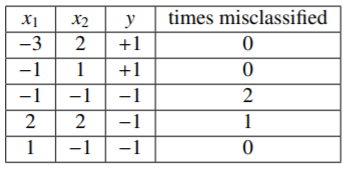
\includegraphics{perceptron.PNG}
\captionof{figure}{Training Data}
\label{fig:table}
\end{center}
\end{minipage}
\begin{parts}
\part
\begin{subparts}
\subpart[3] Assume that the initial weight is $w^{(0)} = [-3,2,1]$ where $1$ is the offset term. So the feature $x_3 = 1$ is constant. What is the equation of the separating line expressed in terms of $x_1$ and $x_2$ determined by the algorithm ?
\begin{solutionorbox}[1.5in]

\end{solutionorbox}
\subpart[1] In some cases, removing a single point can change the decision boundary. Here would removing a single point from the training set change the decision boundary? Please explain your answer.
\begin{solutionorbox}[1.4in]

\end{solutionorbox}
\subpart[2] If we added the point $[2,-2]$ with label $+1$ to the training set, then would we obtain different results? In particular, would the algorithm converge? 
\begin{solutionorbox}[1in]

\end{solutionorbox}
\end{subparts}

\begin{minipage}{0.3\textwidth}
Figure \ref{fig:svm3} shows training data with two classes. We want to use hard-margin support vector machine. Remember that we choose the decision boundary to maximize the margin. 
\end{minipage}
\begin{minipage}{0.75\textwidth}
\begin{center}
    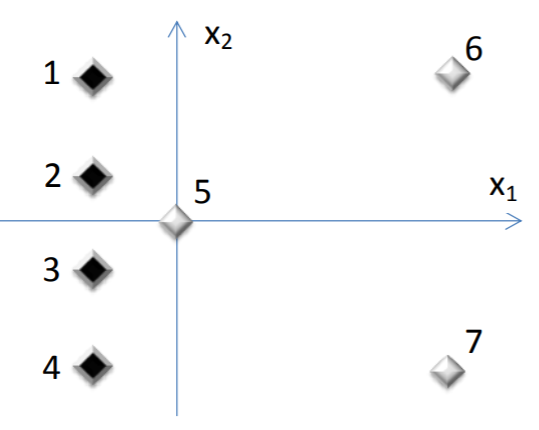
\includegraphics[scale=0.92]{svm2.PNG}
    \captionof{figure}{Training Data}
\label{fig:svm3}
\end{center}
\end{minipage}

\part
\begin{subparts}
\subpart[2] Draw the decision boundary obtained by the hard-margin SVM method with a solid line. Draw the margins on either side with 
dashed lines. 
\subpart [1] What are the \textbf{possible} support vectors. Please indicate the number.
\begin{solutionorbox}[1in]

\end{solutionorbox}
\subpart[1] What is the classification error on the training set? In other words, how many points are incorrectly classified?
\begin{solutionorbox}[1in]

\end{solutionorbox}
\subpart[1] Would the removal of a single point change the decision boundary? If so, then what points?
\begin{solutionorbox}[1in]

\end{solutionorbox}
\subpart[1] Suppose we use leave-one-out cross validation meaning we use 7-fold cross validation with a split of 6 to 1 between training set and validating set. Compute the average classification error over the 7-folds.
\begin{solutionorbox}[1.1in]

\end{solutionorbox}
\end{subparts}
\end{parts}


\end{questions}


\end{document}
